% !TeX root = ../thesis.tex

\chapter{Introduction}
\label{sec:introduction}

%\gls{ma} \gls{online_reference}

This chapter provides a brief introduction to the topic and highlights motivation for the chosen task. It further outlines the research questions contemplated
 during the course of presented work.
%\cite{Stiller2015}


\section{Motivation}

Computer vision has received a lot of attention from research communities specially 
after the advent of deep learning based approaches. Autonomous driving in particular can
leverage such recently developed learning based computer vision methods for perception
of the environment. Semantic segmentation is a task in computer vision where each 
pixel in an image is assigned to a predefined category label (\textit{person, bicycle, car etc}) as shown in \ref{fig:semseg}.
Although, semantic segmentation plays a key role in efficient and holistic semantic 
representation of the scene under observation however highly complex and dynamic situations 
such as urban scenarios which involve multiple traffic participants demand 
an even fine-grained instance-level understanding of the scene. 
Instance segmentation on the other hand deals with delineating each distinct object 
of interest appearing in an image without providing necessary semantic layout information about the scene \ref{fig:instseg}.
\begin{figure}[!ht]
%\centering
    \subfigure[RGB Image]{
        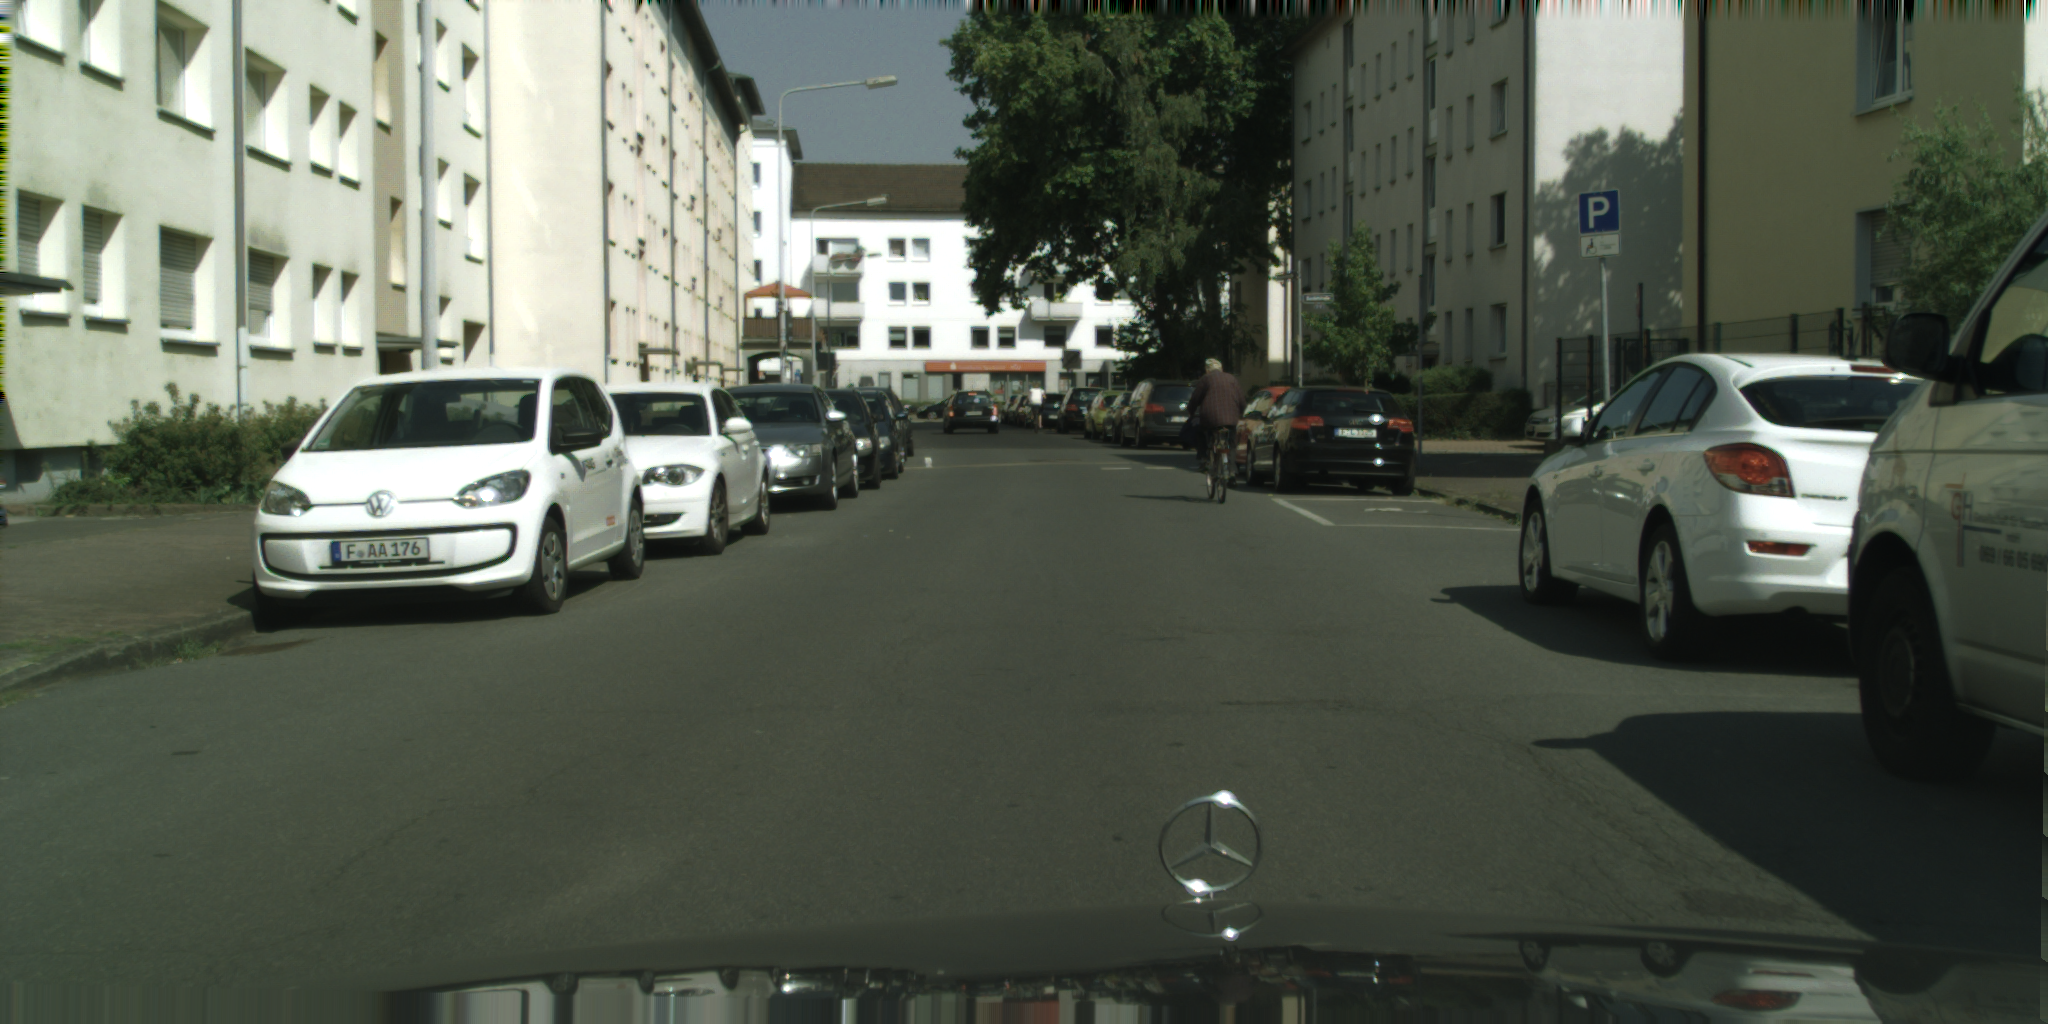
\includegraphics[width = \textwidth / 2 ]{Graphics/Introduction_images/frankfurt_000000_000576_leftImg8bit}
        \label{fig:RGBimage}}
    %\hspace{1pt}
     %add desired spacing between images, e. g. ~, \quad, \qquad, \hfill etc.
     %(or a blank line to force the subfigure onto a new line)
    \subfigure[Semantic Segmentation]{
        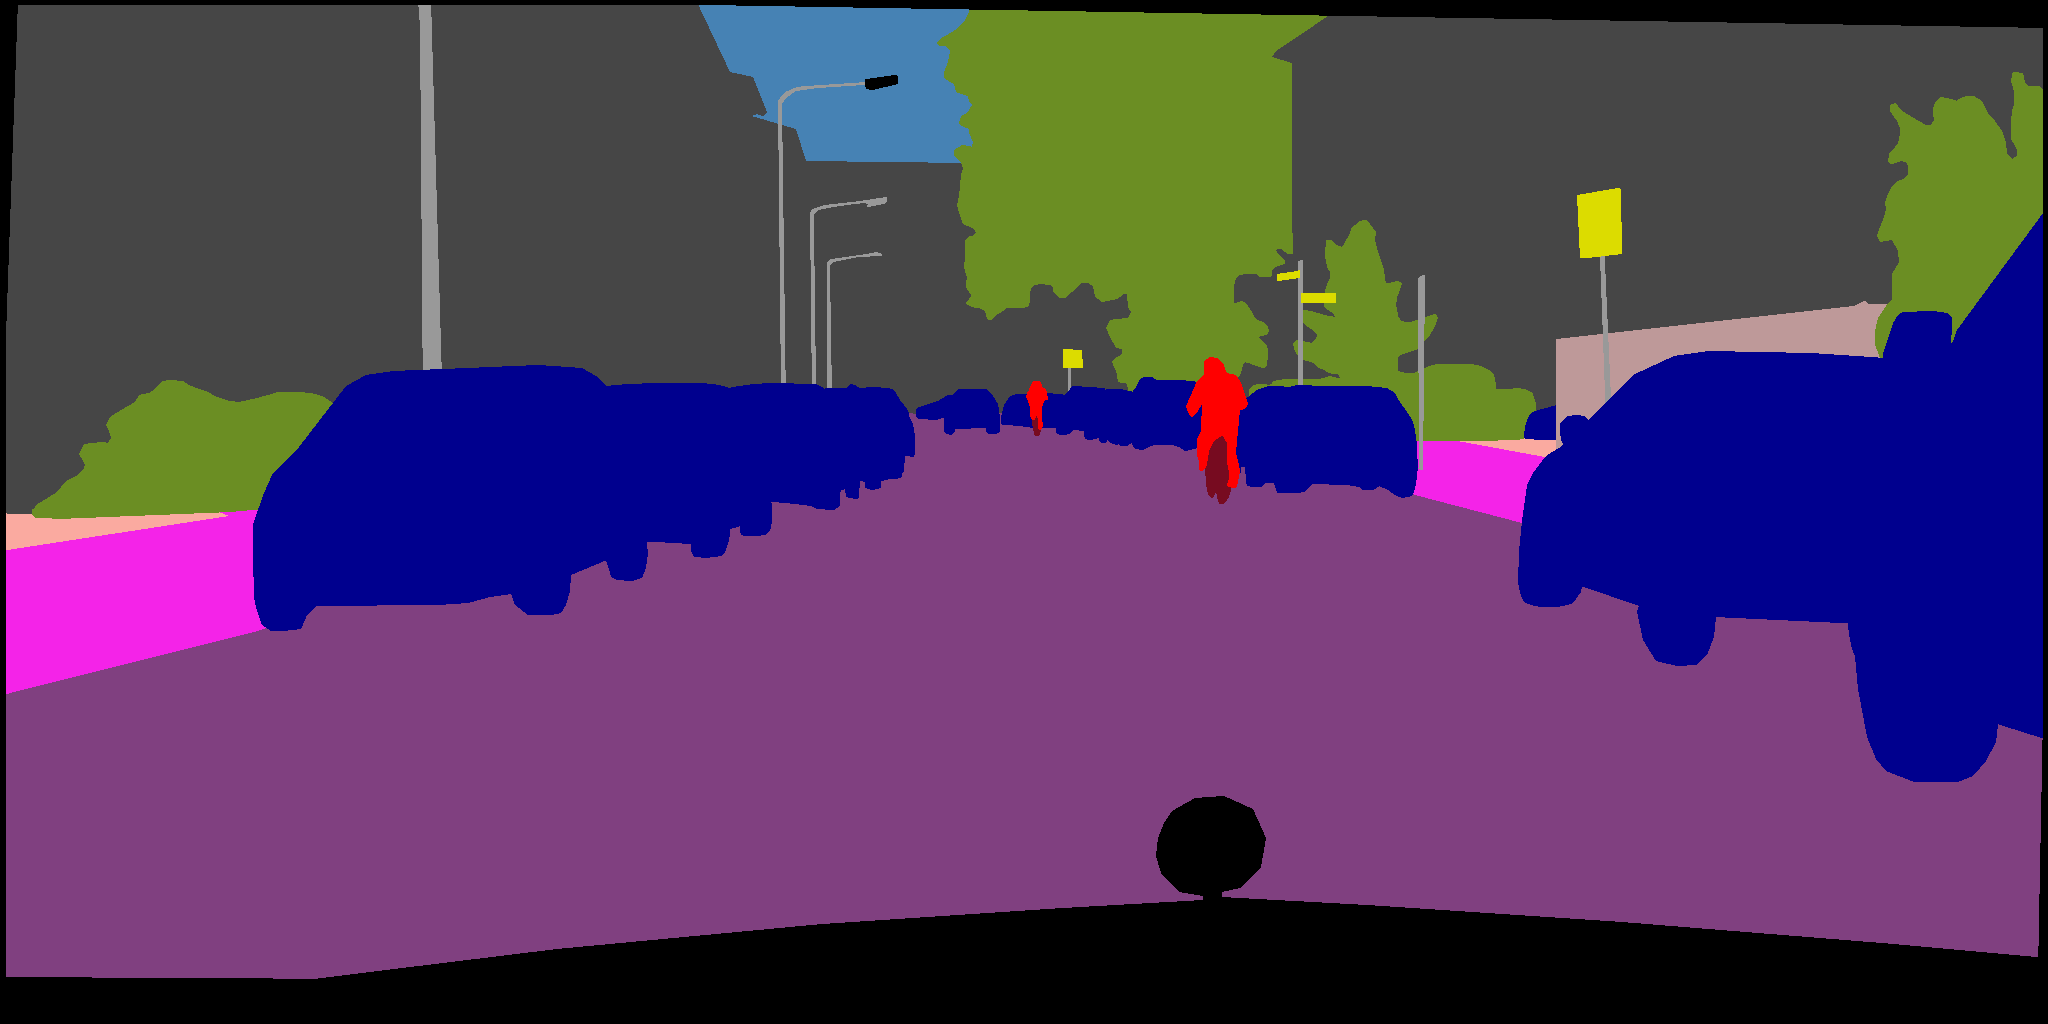
\includegraphics[width = \textwidth / 2 ]{Graphics/Introduction_images/frankfurt_000000_000576_gtFine_color}
        \label{fig:semseg}}
    \subfigure[Instance Segmentation]{
        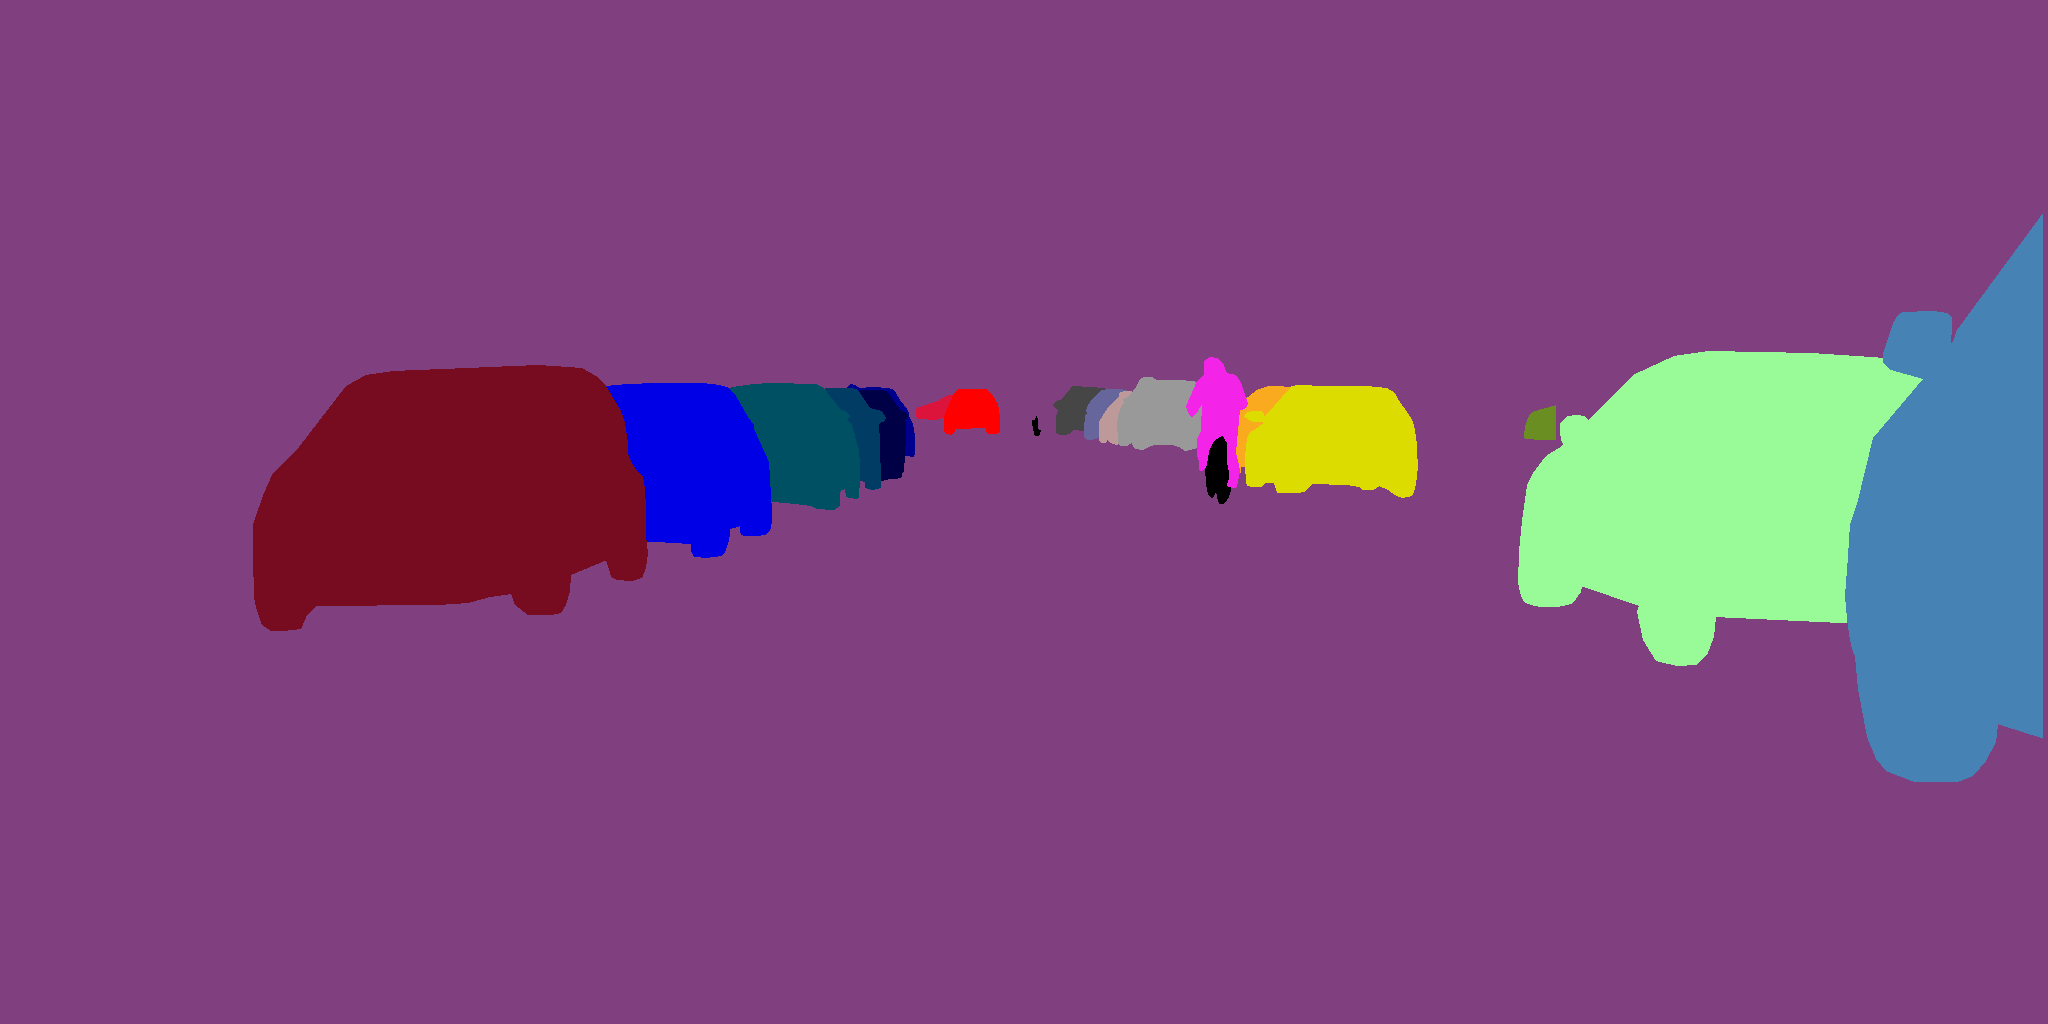
\includegraphics[width = \textwidth / 2 ]{Graphics/Introduction_images/Instance_seg}
        \label{fig:instseg}}
%   \hspace{1pt}
    \subfigure[Panoptic Segmentation]{
        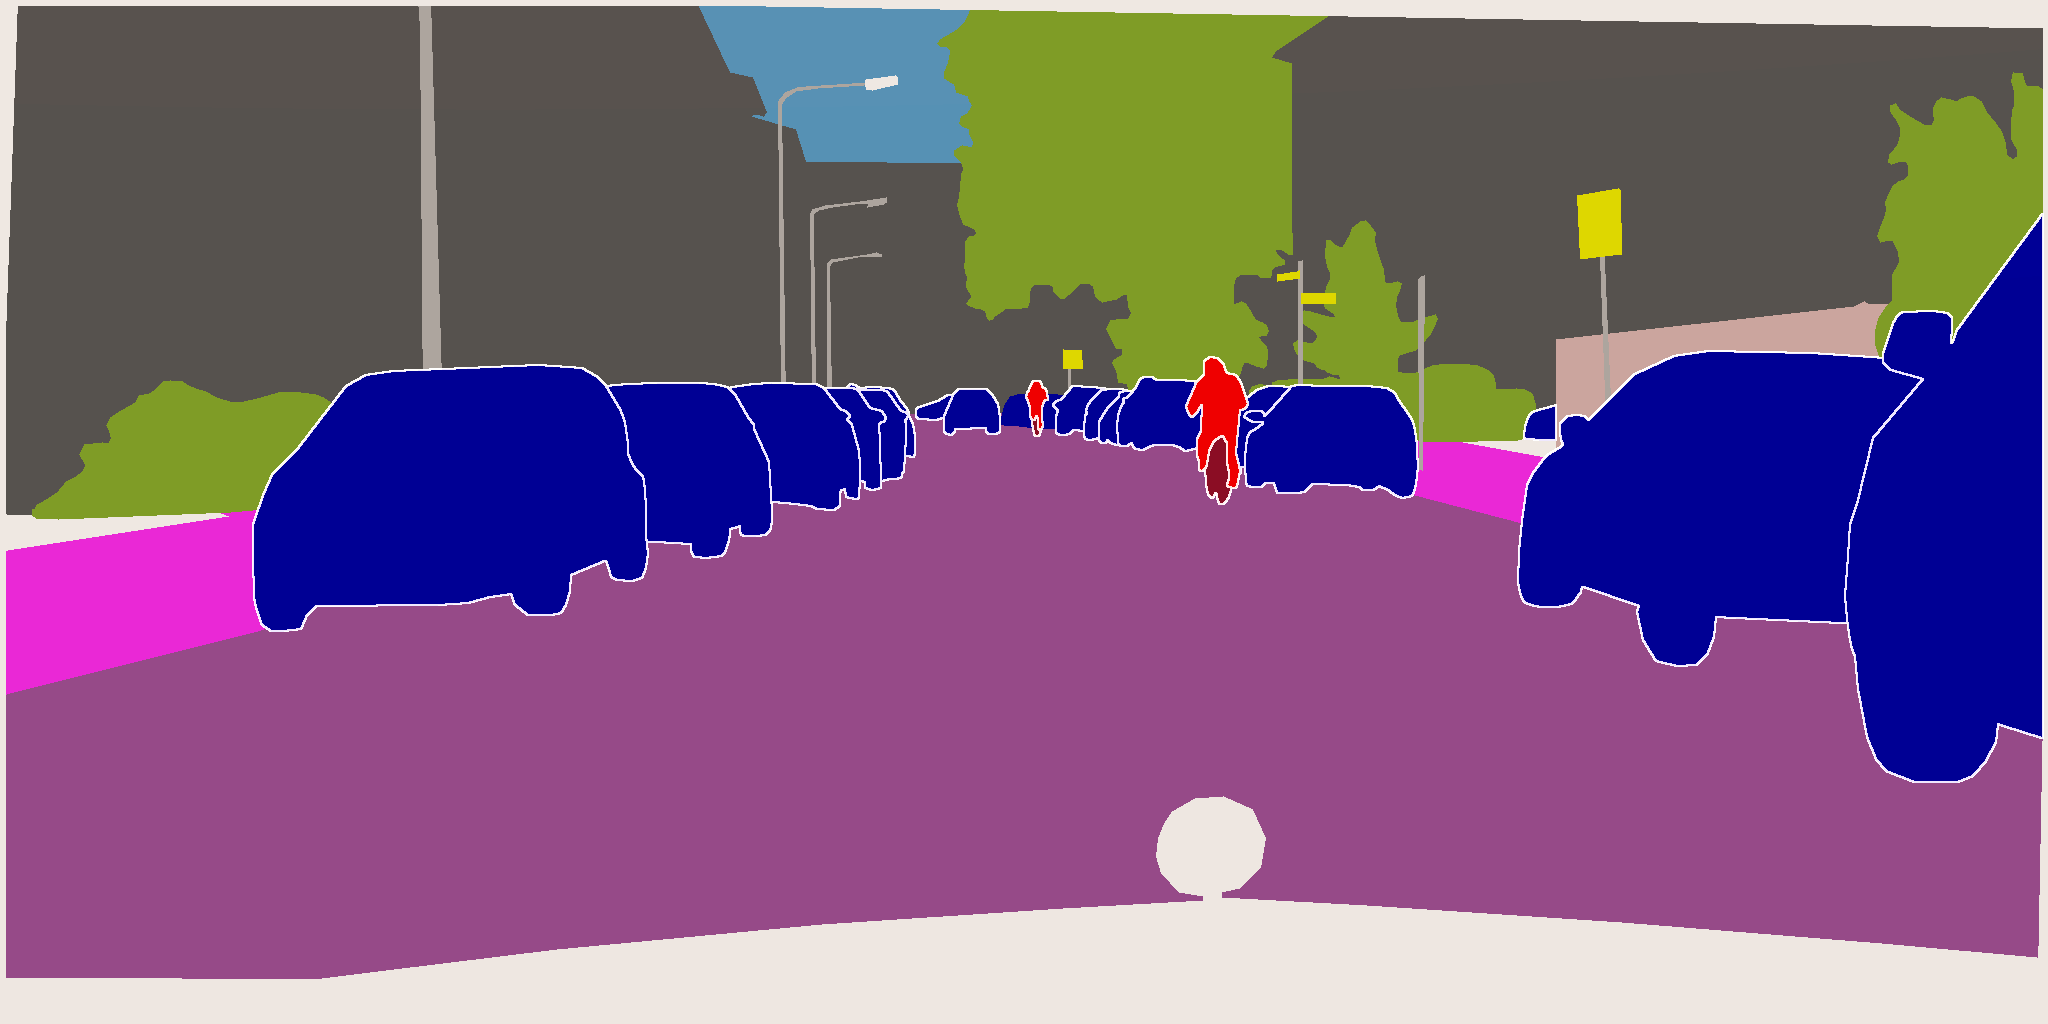
\includegraphics[width = \textwidth / 2 ]{Graphics/Introduction_images/Pansegbright}
        \label{fig:panseg}}
    \caption[Image Segmentation approaches] {Image and corresponding representations a) depicts an RGB image taken from driver's perspective b) shows semantic segmentation of the RGB image c) represents instance segmentation d) shows panoptic segmentation where semantic segmentation and instance segmentation information is represented in a combined fashion \cite{Cordts2015}}
    \label{fig:Rgbseminstseg}
\end{figure}

\textit {Panoptic segmentation} is a recently proposed segmentation task that aims to combine instance and semantic segmentation in a unified segmentation task to generate rich, coherent and comprehensive scene representation \cite{Kirillov2019}. Panoptic segmentation allows for a representation that describes semantic layout as well individual instances appearing in a single view as depicted in \ref{fig:panseg}. Figure \ref{fig:SemsegZoomed}, shows semantic representation of a common urban scenario where each pixel has been assigned to a given class. Although a useful representation that describes a general layout of the scene by separating road, sidewalk, buildings and other traffic participants but it might not suffice for a satisfactory scene interpretation. Highlighted area in the image shows a blob of red coloured pixels that represent people standing on a sidewalk however it can be difficult to argue about number of people and more importantly if some of them intend to cross the road. On the other hand, figure \ref{fig:PanopticsegZoomed} shows combined representation where the people in highlighted region are further separated as individual instances. Such combined representation gives a much detailed information on the scene and can be leveraged by high-level computer vision tasks to argue about behaviour of traffic participants. Autonomous driving as well other computer vision based applications in robotics and medicine can benefit from such rich multi-modal representation for improved image understanding.

Although, both semantic and instance segmentation can complement each other by providing much more detailed information on the scene, they are fundamentally different in the way they are approached and usually require different network architecture topology. Since panoptic segmentation is a unified segmentation task and both of the aforementioned tasks usually rely on features learned using \gls{cnns} it seems a reasonable choice to tailor the architecture by augmenting a common feature extractor. This common feature extractor backbone could learn features that can be utilized by the network to generate instance and semantic segmentation in a combined fashion. Most of the state-of-the-art methods that attempted to solve panoptic segmentation task within a single network either use top-down approaches or proposal based methods such as Mask R-CNN \cite{He2017}. One problem with such two-stage methods is their requirement for an additional region proposal network and furthermore they generate overlapping instance masks with ambiguous instance boundaries which demand additional conflict resolving methods.

\begin{figure}[!ht]
%\centering
    \subfigure[Semantic Segmentation]{
        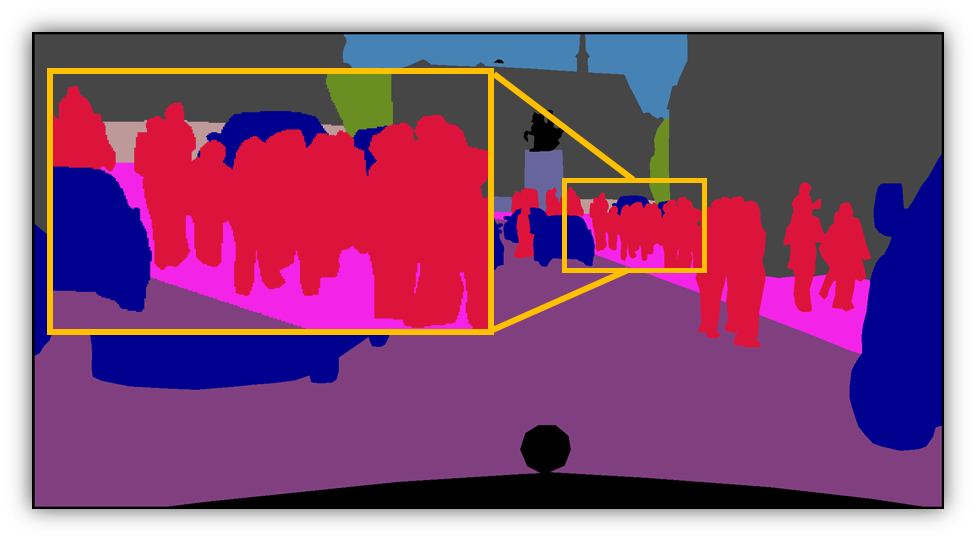
\includegraphics[width = \textwidth / 2 ]{Graphics/Introduction_images/SemsegZoomed.png}
        \label{fig:SemsegZoomed}}
    %\hspace{1pt}
     %add desired spacing between images, e. g. ~, \quad, \qquad, \hfill etc.
     %(or a blank line to force the subfigure onto a new line)
    \subfigure[Panoptic Segmentation]{
        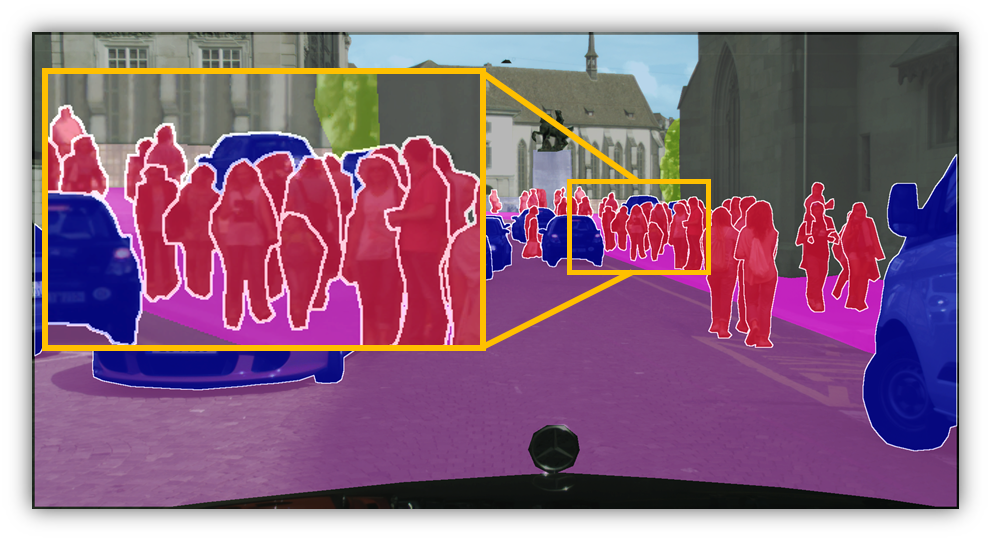
\includegraphics[width = \textwidth / 2 ]{Graphics/Introduction_images/PanopticsegZoomed.png}
        \label{fig:PanopticsegZoomed}}
            \caption[Semantic and Panoptic Segmentation] {Figure shows semantic and panoptic segmentation of an urban scene - highlighting the additional information facilitated by panoptic segmentation a) depicts semantic segmentation of an urban scene b) shows corresponding panoptic segmentation of the scene taken from Cityscapes dataset \cite{Cordts2015}}
\end{figure}





Therefore, it is desired to investigate a simple panoptic segmentation architecture that utilizes dense features extracted from a common backbone feature extractor and makes use of these features to generate both instance and semantic segmentation modalities in a multi-task setting. It is also desired to achieve instance segmentation by exploiting pixel-level relationships whereby learning center points and extent of each instance in one step instead of generating region proposal based overlapping instance masks. 

\section{Problem Statement}

This thesis addresses the task of panoptic segmentation for urban scenarios. The goal
of panoptic segmentation is to assign a unique value, encoding both semantic label and instance id, to every pixel in an image. In panoptic segmentation task, classes are divided into two main categories:

\begin{itemize}
  \item \textit{Stuff}  – amorphous regions of similar texture or material such as sky, building, road.
  \item \textit{Things} – countable objects such as people, cars, bicycles.
\end{itemize}

It is required to identify the class label and extent of each instance of  \textit{things} classes, and only a class labels for all pixels belonging to \textit{stuff} classes. Moreover, it is desired to learn and generate both instance and semantic segmentation modalities within a single network architecture.

In this context, the presented work aims to answer following questions:

\begin{enumerate}

	\item  How to pose two fundamentally diverged approaches in a unified multi-task setting?
	\item  How to represent instances and their pixel-level relationships to generate instance segmentation?

\end{enumerate}

Furthermore, it is desired to investigate instance encoding possibilities and study effects of these representations on overall panoptic segmentation task. 


\section{Outline}
This thesis is structured as follows - Chapter 2 provides a brief overview of fundamentals in semantic, instance and panoptic segmentation. Related work and corresponding literature review has been discussed in chapter 3. In chapter 4, various data representations are introduced and analyzed in the context of pixel-level instance encoding. Subsequently Chapter 5 describes network architecture and experimental setup. In chapter 6, a structured approach to generate panoptic segmentation has been briefly explained. Chapter 7 analyzes the experimental results obtained through these approaches considering both qualitative and quantitative evaluations. Finally, chapter 8 summarizes the thesis and provides an outlook regarding future work.